% \documentclass[preprint]{elsarticle}
%% Use the option review to obtain double line spacing
\documentclass[preprint,review,12pt]{elsarticle}

%% Use the options 1p,twocolumn; 3p; 3p,twocolumn; 5p; or 5p,twocolumn
%% for a journal layout:
%% \documentclass[final,1p,times]{elsarticle}
%% \documentclass[final,1p,times,twocolumn]{elsarticle}
%% \documentclass[final,3p,times]{elsarticle}
%% \documentclass[final,3p,times,twocolumn]{elsarticle}
%% \documentclass[final,5p,times]{elsarticle}
% \documentclass[final,5p,times,twocolumn]{elsarticle}
\usepackage{lineno}
\usepackage{hyperref}
\usepackage{siunitx}
\usepackage{amsmath}
\usepackage{graphicx}
\usepackage{mhchem}
\usepackage{tabularx}
\usepackage{subcaption}
\usepackage{bm}
\linenumbers
\journal{NIM-A}
\begin{document}
\begin{frontmatter}
    \title{Qualification tests of 8-inch MCP-PMTs for JNE}

    \author[a,b,c]{Aiqiang Zhang}%
    \ead{greatofdream@gmail.com}

    \author[a,b,c]{Benda Xu\corref{cor1}}%
    \ead{orv@tsinghua.edu.cn}

    \author[a,b,c]{Jun Weng}
    \author[a,b,c]{Lin Ren}
    \author[a,b,c]{Huiyou Chen}
    \author[a,b,c]{Wenhui Shao}
    \author[a,b,c]{Tong Xu}
    \author[a,b,c]{Zhe Wang}
    \author[a,b,c]{Shaomin Chen}

    \cortext[cor1]{Corresponding author}
    \affiliation[a]{
        organization={Department of Engineering Physics},
        addressline={Tsinghua University}, 
        city={Beijing},
        country={China}}
    \affiliation[b]{
        organization={Center for High Energy Physics},
        addressline={Tsinghua University}, 
        city={Beijing},
        country={China}}
    \affiliation[c]{
        organization={Key Laboratory of Particle \& Radiation Imaging (Tsinghua University), Ministry of Education},
        country={China}}
    \begin{abstract}
The new type of HQE 8-inch MCP-PMTs are used in Jinping Neutrino Experiment of 500t for MeV-scaled neutrino measurements. The detection efficiency of PMTs is significant for resolution. This work presents the implemented testing procedure and the characteristics of a set of sample of PMTs. Result of this work illustrates that detection efficiency of testing PMTs are about 30\%, obviously higher than reference PMT.  
\end{abstract}

\keywords{MCP-PMT, detection efficiency, Jinping Neutrino Experiment}

\end{frontmatter}

\section{Introduction}
% Experiment Introduction and Importance of resolution for Low PE
The Jinping Neutrino Experiment (JNE) of multi-hundred-tons is a large-volume water-based liquid scintillator experiment with \SI{2400}{m} rock overburden \cite{LetterJNE2017} which is under construction. Its main goal is to accurately measure the spectrum of MeV-scale neutrinos, including solar neutrinos, geo-neutrinos, and supernova neutrinos \cite{LetterJNE2017}. % PMT Introduction
The photomultiplier tube (PMT) \cite{HAMAMATSUManual}, which transforms a photon into a single photoelectron (PE), and then to the measurable electric signal, is often used to detect few photons in water Cherenkov detectors \cite{SNO,SuperK} and liquid scintillator detectors \cite{KamLAND,JUNO:2015zny}. The details of the energy spectrum of neutrinos of low energy are determined by the energy resolution, which is dependent on the coverage of light collection and photon detection efficiency of PMTs. The price of PMTs also plays an important role for the coverage of light collection during design. The direction information from Cherenkov photons, which is centered in less than \SI{1}{ns} for electrons less than \SI{30}{MeV}, provides the ability to suppress the background in the solar neutrinos and supernova relic neutrinos measurements for the Cherenkov scintillation detector \cite{Guo_2019}. The short time scale of Cherenkov light requires the deviation of transit time to be less than \SI{1}{ns} considering the uncertainty of about \SI{1.3}{ns} for \SI{10}{m} scale detectors from the dispersion\footnote{The uncertainty from dispersion is estimated as $R\frac{\delta\lambda}{\lambda^2}$, in which $R$, $\delta\lambda$, and $\lambda$ are about \SI{10}{m}, \SI{5}{mm/ns} and \SI{195}{mm/ns} \cite{Luo:2022xrd}.} is the main component.

The new type of 8-inch micro-channel plate PMT (MCP-PMT) (GDB-6082 \cite{GDB-6082}) meeting above requirements including good cost performance, which produced by North Night Vision Science \&Technology (Nanjing) Research Institute Co. Ltd. (NNVT), will be used in JNE. The new type of MCP-PMTs have high collection and quantum effiency\footnote{Photon detection efficiency is the product of collection efficiency and quantum efficiency.}. This work is to confirm the superiority of photon detection efficiency (PDE) and boost on energy resolution of the new type of MCP-PMT. This also is the first measurement for the new type of 8-inch MCP-PMT.

% Testing of Other Experiments
Measurements for the 20-inch MCP-PMT from NNVT, which has a similar structure to 8-inch MCP-PMT, were done by JUNO and confirmed that the average PDE is about 28\% \cite{JUNOMassTesting}. In addition, several other recent PMT characterization tests were reviewed and referenced. Gain, single PE resolution, PDE, transit time spread (TTS), and dark count rate (DCR) are the most important parameters measured in recent different experiments. For example, Daya Bay used 8-inch dynode PMTs (9354KB, R5912, XP1806) \cite{DayaBayTesting}, Double Chooze used 10-inch dynode PMTs (R7081) \cite{DoubleChoozeTesting}, LHAASO used 8-inch dynode PMTs (CR365-02-1) \cite{LHAASOTesting}, HyperKamiokande tested 20-inch dynode PMT (R12860) and MCP-PMT (GDB-6203) \cite{HyperKTesting}, KM3Net used 3-inch dynode PMT(R12199-02) \cite{KM3NetTesting}, XENON1T and XENONnT tested 3-inch dynode PMT (R11410-21) \cite{XENON1TTesting}\cite{XENONnTTesting}, IceCube tested 3-inch PMT (R12199-01) \cite{IceCubeTesting}.

% The structure of paper
This work concentrated on the characteristics of MCP-PMTs in the low photon intensity condition. The setup of the testing system and facility is introduced in sec.~\ref{SetUp}. Detailed analysis methods and results, including Gain, single PE resolution, PDE, TTS, DCR, time characteristics of single electron response (SER), pre-pulse, and after-pulse are described in sec.~\ref{Method}. The boost for energy resolution is discussed in sec.~\ref{Result}. Finally, a summary is given in sec.~\ref{Summary}.

\section{Experimental setup and testing procedure}
\label{SetUp}
\subsection{Reference PMT}
CR365-01\cite{BJBS} and R5912-100\cite{JPBS} from HAMAMATSU are used as reference PMT.
\subsection{Experimental setup}
% Facility
The schema of experimentail facility is shown in Fig~\ref{fig:facility}
\begin{figure}
    % \includegraphics[width=0.8\textwidth]{figure/facility/facility.pdf}
    \caption{The schema of facility}
    \label{fig:facility}
\end{figure}
Light source is a picosecond laser flashing system (PiL040XSM) from Advanced Laser Systems(A.L.S)\cite{NTKLaser}, which can produce short light pulses with a wavelenght of \SI{405}{nm} and a width of \SI{34}{ps}. The light is attenuated by a laser attenuator with 0.5-30db. A fiber splitter with the standard G.657.A1 distributes attenuated light into 4 channels, which face directly to the top of PMT.

A black plastic box acts as darkroom splitted into 4 grids. Each grid holds a PMT and is equipped with an end of splitter channel. CAEN V1751 10-bit digitizer with 1GHz sample rates is used for data taking\cite{CAENV1751}, which controlled by a custom-made data acquisition(DAQ) software based on CAEN library. The offset of digitizer is set to about \SI{0.183}{V} and the dynamic range is from \SI{-0.817}{V} to \SI{0.183}{V}. Wiener EDS 30330p high voltage(HV) module\cite{WIENERHV} supplies a positive voltage for each PMT. Bare PMTs are connected to the HV module and digitizer with a pluggable HV divider with an integrated HV-signal decoupler. The HV divider is soldered to potted PMTs with HV and signal interfaces seperated. 

LEMO line and HV line are go through an \SI{0.5}{cm} hole of the box and directly connected HV divider with HV module and digitizer. 

\subsection{Testing procedure}
All PMTs were measured under the HV provided by the vendor(NNVT), which are calibrated at the gain of $1\times10^7$. To stabilize and reduce the influence of the dark noise, all pmts stayed in darkroom  with HV on for 10 hours before DAQ started. DAQ sampling contains two stage: the first stage is noise stage and DAQ works without laser and triggered periodly at 1kHz mainly for DCR calculation; the second stage is laser stage, in which DAQ sample data with laser and triggered by the output of trigger from laser for other characterization.
\sisetup{separate-uncertainty=true}
\sisetup{multi-part-units=single}
\section{Methods and results}
\label{Method}
% The setup of the experiment and preanalysis are discussed in Section~\ref{sec:laserstage}. Analysis method and results of parameters are introduced in the following sections.
\subsection{Preanalysis}
\label{sec:laserstage}

The laser intensity is adjusted to the level of $1/20$ occupancy to obtain single PE events. The window size $T_{\mathrm{wave}}$ is \SI{10400}{ns} to include all the possible after-pulses (see Section~\ref{sec:afterpulse}). The rising edge of the trigger waveform from the laser system is linearly interpolated to get the half-height time $t_{\mathrm{trig}}$ at about \SI{200}{ns}, as shown in Fig.~\ref{fig:triggertime}.
\begin{figure}[!htbp]
    \centering
    \includegraphics[width=\LF\textwidth]{figures/method/triggerwave.pdf}
    \caption{An example of PMT and trigger signals. The orange line is the trigger waveform, with its high and low voltages indicated by two black horizontal dashed lines. The green cross is the interpolated trigger time $t_{\mathrm{trig}}$. The solid blue line is the PMT waveform with a PE pulse. The horizontal violet dotted line is the voltage threshold for calculating the baseline shown by the blue horizontal dashed line. The black horizontal dash lines intersect 10\%, 50\% and 90\% of (downward) rising and falling edges. The red and yellow vertical dashed lines are for the 10\% rising edge and the pulse peak respectively.}
    \label{fig:triggertime}
\end{figure}


In the preanalysis, we select a preliminary window $[t_{\mathrm{trig}},600\,\mathrm{ns}]$ where dark noises (\SI{\sim 10}{kHz} in Section~\ref{sec:dcr}) and laser pulses are expected to contribute 0.004 and 0.05 counts on average. The peak time $t_p$ is the minimum position in each window, as shown in Fig.~\ref{fig:triggertime}.
%Because the maximum pulse is selected in each waveform, the expected charge distribution is the distribution of $\max(C_n)$ ($n=1,...,N$), in which $C_n$ is the charge of the nth PE and $N$ is the number of PE in a waveform.


The nonzero baseline is estimated from the sidebands $[-200\,\mathrm{ns},-10\,\mathrm{ns}]$ and $[100\,\mathrm{ns},200\,\mathrm{ns}]$ relative to $t_p$. % padding
To remove potential additional pulses in the sidebands, as the horizontal violet dotted line in Fig.~\ref{fig:triggertime} we define a voltage threshold from a rough estimation of white noise and cut off additional \SI{10}{ns} around each over-threshold time interval. The baseline $\mu_b$ is estimated as the average of the residual sidebands. The peak height $V_p$ of a pulse is the difference between $\mu_b$ and the minimum voltage.

Over all the waveform samples, a Gaussian $f(t;t_0,\sigma_{t0}^2)$ is fitted to the distribution of $t_p-t_{\mathrm{trig}}$ of pulses whose $V_p$ exceeds \SI{5}{ADC}. We define a new candidate window, about \SI{30}{ns} long, as $[t_0-5\sigma_{t0}, t_0+5\sigma_{t0}]$ to calculate new $t_p$ and $V_p$ by repeating the above procedures.  With such a candidate window the dark counts reduced by 10, we shall conduct the charge and time characterization of the single PE in the following sections.

\subsection{Single-PE charge spectrum and resolution}
\label{sec:noisepeak}

Considering the rise and fall time distributions, the charge $Q$ of a pulse is defined as % padding
the summation of the baseline-subtracted voltages in a time window $[\SI{-10}{ns}, \SI{75}{ns}]$ relative to $t_p$ as illustrated in the pink region of Fig.~\ref{fig:triggertime}. The input impedance being \SI{50}{\Omega}~\cite{CAENV1751}, the charge in the unit of Coulomb is $Q/\SI{50}{\Omega}$.

Such $Q$ in Fig.~\ref{fig:triggercharge} represents the charge of a single PE with negligible multi-PE contributions due to the low occupancy. A long tail is evident in the single-PE charge distribution, also found in the NNVT 20-inch MCP-PMTs by the JUNO collaboration~\cite{JUNOMassTesting}. Zhang~et~al.~\cite{JUNOLongtail} proposed a phenomenological parameterization without dedicated consideration of the multiplication process of the PEs. Our future publications will discuss the physical model and solution of the long tail.

To describe the peak shape of the $Q$ distribution, a Gaussian function $f(Q;Q_0,\sigma^2_{Q_0})$ is fitted to the interval $[0.65Q_0, 1.35Q_0]$ via the modified least-square (MLS)~\cite{Cowan1998StatisticalDA} as the red line in Fig.~\ref{fig:triggercharge}. To remove the influence of the pedestal and describe the long tail~\cite{JUNOLongtail}, pulses with $V_p>\SI{3}{ADC}$ and $Q>0.25Q_0$ are selected to calculate the mean $\overline{Q}$ and sample variance $s^2_{Q}$ of $Q$.
% The $V_p$ distribution with \SI{1}{ADC} bin width in Fig.~\ref{fig:triggerpeak} 
The two cuts are complementary to exclude some noises with small $V_p$ but large $Q$~(Fig.~\ref{fig:triggercharge}).

\begin{figure}[!htbp]
    \centering
    \begin{subfigure}[b]{\SF\textwidth}
        \includegraphics[width=\textwidth]{figures/method/triggercharge.pdf}
        \caption{}%PM
        \label{fig:triggercharge}
    \end{subfigure}
    \begin{subfigure}[b]{\SF\textwidth}
        % \includegraphics[width=\textwidth]{figures/method/triggerpeak.pdf}
        % \caption{}%PM
        % \label{fig:triggerpeak}
        \includegraphics[width=\textwidth]{figures/result/gainres.pdf}
        \caption{}
        \label{fig:totalchargeCompare}
    \end{subfigure}
    \caption{(\subref{fig:triggercharge}) The long-tailed single-PE charge distribution of an MCP-PMT. The entries around zero are waveforms with no signal. The vertical blue dashed line is the pedestal cut. The orange histogram is the selected waveforms with peak-height cut ($V_p>\SI{3}{ADC}$). The pink and green areas are the fit intervals for the peak and valley parameters. (\subref{fig:totalchargeCompare}) The charge and resolution ratios show the effect of the long tail. The point and crosses represent the reference and MCP PMTs, respectively.
    }
\end{figure}

The gains of the main peak and the entire sample are ${Q_0}/({\SI{50}{\Omega}} e) \approx \num{e7}$ and ${\overline{Q}}/(\SI{50}{\Omega} e)$, $e$ being the charge of an electron. The relative \emph{peak} and \emph{sample resolutions} $\nu_0$ and $\nu$ are defined as ${\sigma_{Q_0}}/{Q_0}$ and ${\sqrt{s^2_{Q}}}/{\overline{Q}}$.  Shown in Fig.~\ref{fig:totalchargeCompare}, $\overline{Q}$ is about 1.8 times $Q_0$ for the MCP-PMTs, in agreement with Zhang~et~al.~\cite{JUNOLongtail}. The long tail worsens the resolution of MCP-PMTs from $\nu_0=\num{0.25 \pm 0.02}$ to $\nu=\num{0.69 \pm 0.03}$, but is less pronounced for the reference dynode PMT.

\subsection{Peak-to-valley ratio}
\label{sec:PV}
A parabolic function is fitted to the valley based on MLS in the interval $[-0.15Q_0, 0.25Q_0]$ relative to the least-counted bin of the histogram between the pedestal and the main peak, as shown in Fig.~\ref{fig:triggercharge}. The \emph{valley count} $N_v$ is defined as the minimum of the parabola and \emph{peak count} $N_p$ is the maximum of the Gaussian described in Section~\ref{sec:noisepeak}. The peak-to-valley ratio~(P/V) ${N_p}/{N_v}$ shows the ability to discriminate between electronic noises and a PE signal. The average P/V of MCP-PMTs is about 5.8, significantly higher than that (about 2.4) of the reference PMT.

\subsection{Single electron response}
\label{sec:SER}
As shown in Fig.~\ref{fig:triggertime}, $t^{10}_r$, $t^{50}_r$, $t^{90}_r$ ($t^{10}_f$, $t^{50}_f$, $t^{90}_f$) are the times of interpolated 10\%, 50\%, and 90\% $V_p$ in the rising (falling) edge. We define the rise time $t_r = t^{90}_r - t^{10}_r$, fall time $t_f = t^{10}_f - t^{90}_f$ and full width at half maximum $\mathrm{FWHM} = t^{50}_f - t^{50}_r$ to describe the shape of \emph{single electron response}~(SER).  They are measured to be $t_r = \SI{3.71\pm0.15}{ns}$, $t_f = \SI{15.6\pm1.8}{ns}$ and $\mathrm{FWHM} = \SI{9.07\pm0.63}{ns}$ for the 9 MCP-PMTs.

% \begin{figure}
%     \centering
%         \includegraphics[width=\MF\textwidth]{figures/method/triggerSER.pdf}
%         \caption{A fitting result of a pulse.}%PM
%         \label{fig:triggerser}
    % \begin{subfigure}[b]{\SF\textwidth}
    %     \includegraphics[width=\textwidth]{figures/result/tausigma.pdf}
    %     \caption{}%PM
    %     \label{fig:sigmaCompare}
    % \end{subfigure}
    % \caption{(a)  (b) $\tau$ versus $\sigma$ of 9 MCP-PMTs.}
% \end{figure}
To get a smooth SER, signals with $V_p>\SI{3}{ADC}$, $Q \in [0.5Q_0, 1000\mathrm{ADC\cdot ns}]$ and $\mathrm{FWHM} \in [2\,\mathrm{ns}, 15\,\mathrm{ns}]$ are selecteed to exclude the noise and large pulses. %padding
An \emph{exGaussian} distribution $f^N(t;\mu_{\mathrm{SER}},\sigma_\mathrm{SER}^2)\otimes f^{\mathrm{Exp}}(t;1/\tau_\mathrm{SER})$~\cite{Luo:2022xrd} is used to fit the SER% as shown in Fig.~\ref{fig:triggerser}
, in which $\mu_{\mathrm{SER}}$ is the time offset of the pulse, $\sigma_{\mathrm{SER}}$ and $\tau_{\mathrm{SER}}$ model the shape of SER. They are measured to be $\tau_{\mathrm{SER}} = \SI{7.2\pm1.0}{ns}$ and $\sigma_{\mathrm{SER}} = \SI{1.62\pm0.06}{ns}$ for the 9 MCP-PMTs.

\subsection{Transit time spread}
\label{sec:TTS}
The PEs from the photocathode drift to the MCP, as shown in Fig.~\ref{fig:mcpelectron}. The drifting electric field and the PE trajectory are simulated by a simplified model consisting of a cathode at \SI{0}{V}, a focusing electrode at \SI{480}{V} and an MCP at \SI{528}{V}. The PEs from the top of the photocathode with \SI{0}{eV} and \SI{3}{eV} kinetic energies have drift times of about \SI{21}{ns} and \SI{18}{ns}, respectively. A PE entering an MCP channel is multiplied to be an observable pulse, while that hitting the surface of the MCP gets scattered inelastically into several secondary electrons or elastically into one single electron~\cite{Furman}. The scattered electrons drift in the electric field until entering the MCP channels finally to give delayed pulses~\cite{KM3NetTesting}. Multiple secondary electrons with different kinetic energies may cause two or more pulses due to different drift times, as shown in Fig.~\ref{fig:triggerTT2pulse}.

\begin{figure}[!htbp]
    \centering
    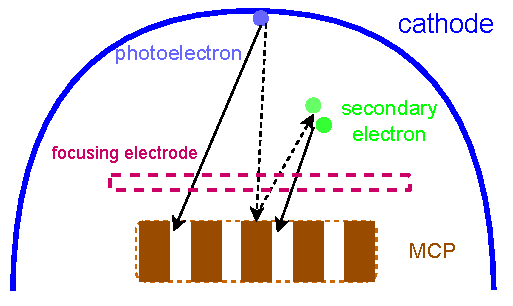
\includegraphics[width=\MF\textwidth]{figures/method/MCPelectron.pdf}
    \caption{The PEs drift from the photocathode to the MCP and get amplified or scattered.}%PM
    \label{fig:mcpelectron}
\end{figure}

The transit time (TT) of a PE is the time needed to travel from the photocathode to the anode, mainly composed of the drift and multiplication times. However, the absolute TT is hard to measure. A relative $\mathrm{TT}$ is defined as the time difference between the trigger signal $t_{\mathrm{trig}}$ and 10\% of the rise time of a PE pulse $t_r^{10}$. The $\mathrm{TT}$ distribution of the MCP-PMTs contains slowly rising and falling edges on both sides of the peak, as shown in Fig.~\ref{fig:triggerTTSLog}. The rising edge is due to the PEs with larger kinetic energies, while the falling one consists of secondary electrons with longer drift times~\cite{longtail}.

Delayed pulses are searched in the interval $[t_0+20\,\mathrm{ns},t_0+80\,\mathrm{ns}]$ to separate them from the main pulses in $[t_0-5\,\mathrm{ns},t_0+5\,\mathrm{ns}]$. The blue histogram in Fig.~\ref{fig:triggerTTlatepulse} is the distribution of the delayed pulses, and the filled one is for those with the main pulses in the same waveform, an example demonstrated in Fig.~\ref{fig:triggerTT2pulse}. The sharp difference between them at about \SI{40}{ns} after the main peak, twice the drift time of PEs from the cathode to the MCP, reasonably illustrates that an elastically scattered electron cannot appear together with a main pulse in a waveform.

\begin{figure}[!htbp]
    \centering
    \begin{subfigure}[t]{\SF\textwidth}
        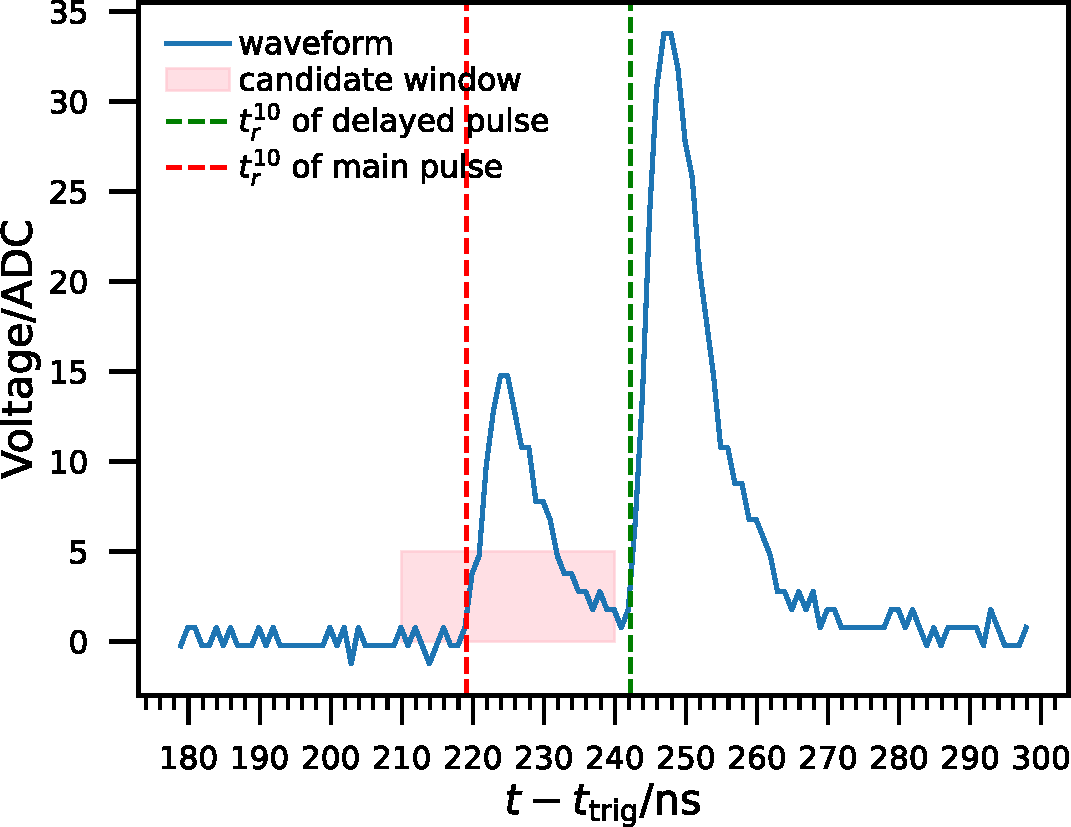
\includegraphics[width=\textwidth]{figures/method/triggerDoublePulse.pdf}
        \caption{}%PM
        \label{fig:triggerTT2pulse}
    \end{subfigure}
    \begin{subfigure}[t]{\SF\textwidth}
        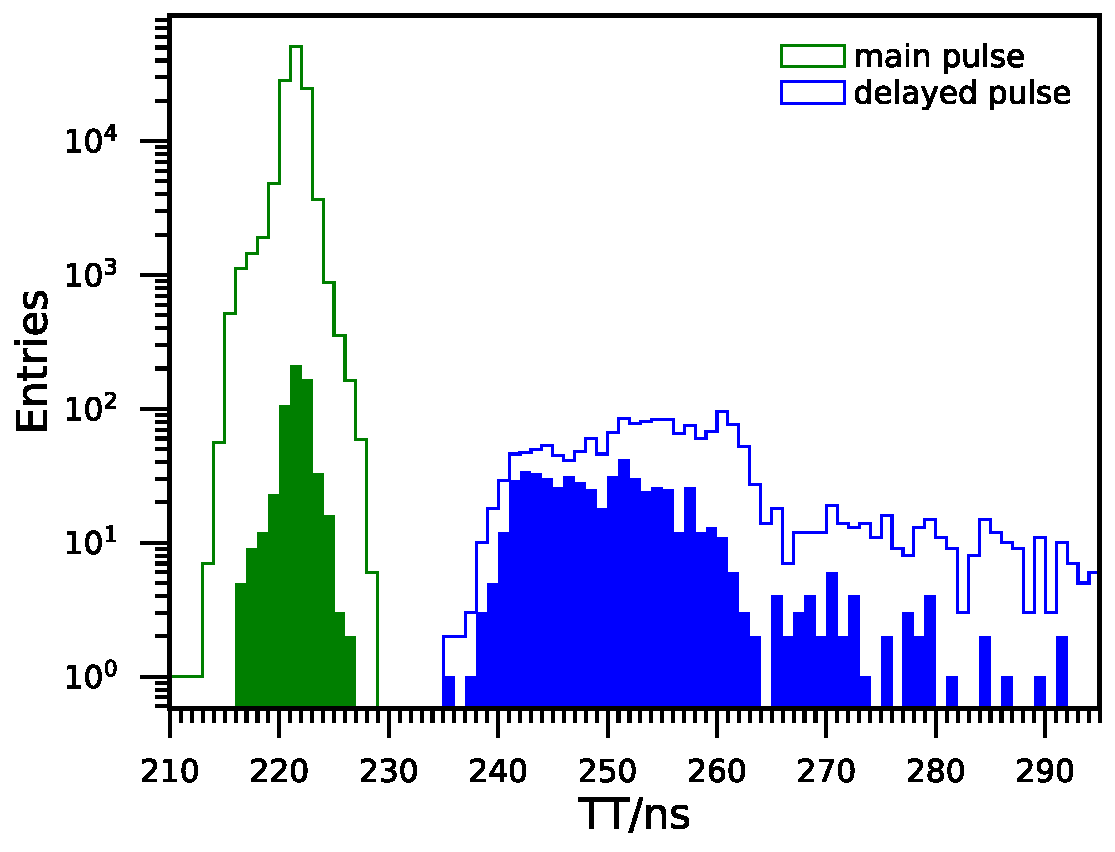
\includegraphics[width=\textwidth]{figures/method/triggerDelayedPulse.pdf}
        \caption{}%PM
        \label{fig:triggerTTlatepulse}
    \end{subfigure}
    \caption{(a) Double-pulse example. The first pulse falls in the candidate window defined in Section~\ref{sec:laserstage}. (b) The green and blue histograms are the main and delayed pulse distributions, respectively. The filled histograms are waveforms containing the main and delayed pulses simultaneously.}
\end{figure}

The main and early components are modeled with Gaussian functions % padding
$N_1f_1^N(t;\mu_{\mathrm{TT}},\sigma_{\mathrm{TT}}^2)$ and $N_2f_2^N(t;\mu_K,\sigma_K^2)$, the subscript $K$ standing for PEs with high kinetic energies. Considering the exponential distribution of kinetic energies of secondary electrons~\cite{Furman,SecondElectron}, $f^\mathrm{Exp}(t;1/\tau_S)$ is suitable to model the delayed component.  A more comprehensive measurement is ongoing.  We artificially add a constant $b_S$ and a translation of $\mu_{TT} + 3\sigma_{TT}$ to fit the data. As shown in Fig.~\ref{fig:triggerTTSLog}, the \SI{0.5}{ns}-binned histogram of $\mathrm{TT}$ is fitted by

\begin{equation}
    \begin{aligned}
        B&+N_1f_1^N(t;\mu_{\mathrm{TT}},\sigma_{\mathrm{TT}}^2)\\
        &+N_2f_2^N(t;\mu_K,\sigma_K^2)\\
        &+b_SH(\mu_{\mathrm{TT}}+3\sigma_{\mathrm{TT}})+N_Sf^{\mathrm{Exp}}\left(t-(\mu_{\mathrm{TT}}+3\sigma_{\mathrm{TT}});\frac{1}{\tau_S}\right)
    \end{aligned}
\end{equation}
in which $H$ is the Heaviside function to limit the definition domain of the delayed component, and $B$ is the constant dark noise rate. The early and exponential components can be omitted in a rough simulation due to their small ratios in the 9 MCP-PMTs: $N_2/N_1 = \num{0.042\pm0.013}$, $N_S/N_1 = \num{0.014\pm0.002}$ and $2b_S\sigma_{\mathrm{TT}}/N_1 l= \num{0.00028\pm0.00005}$.  $\sigma_K$, $\tau_S$ and $\mu_{\mathrm{TT}}-\mu_K$ are fitted to be $\SI{1.4 \pm 0.3}{ns}$, $\SI{1.1\pm 0.1}{ns}$ and $\SI{3.2\pm 0.2}{ns}$. TTS ($\SI{1.74\pm0.05}{ns}$) is defined as FWHM$=2\sqrt{2\ln 2}\sigma_{\mathrm{TT}}$~\cite{HAMAMATSUManual} representing the timing resolution. The charge and TT seem to have some correlation in Fig.~\ref{fig:triggerTTS2d}, the long tail evident in charge distribution.

\begin{figure}[!htbp]
    \centering
    \begin{subfigure}[t]{\SF\textwidth}
        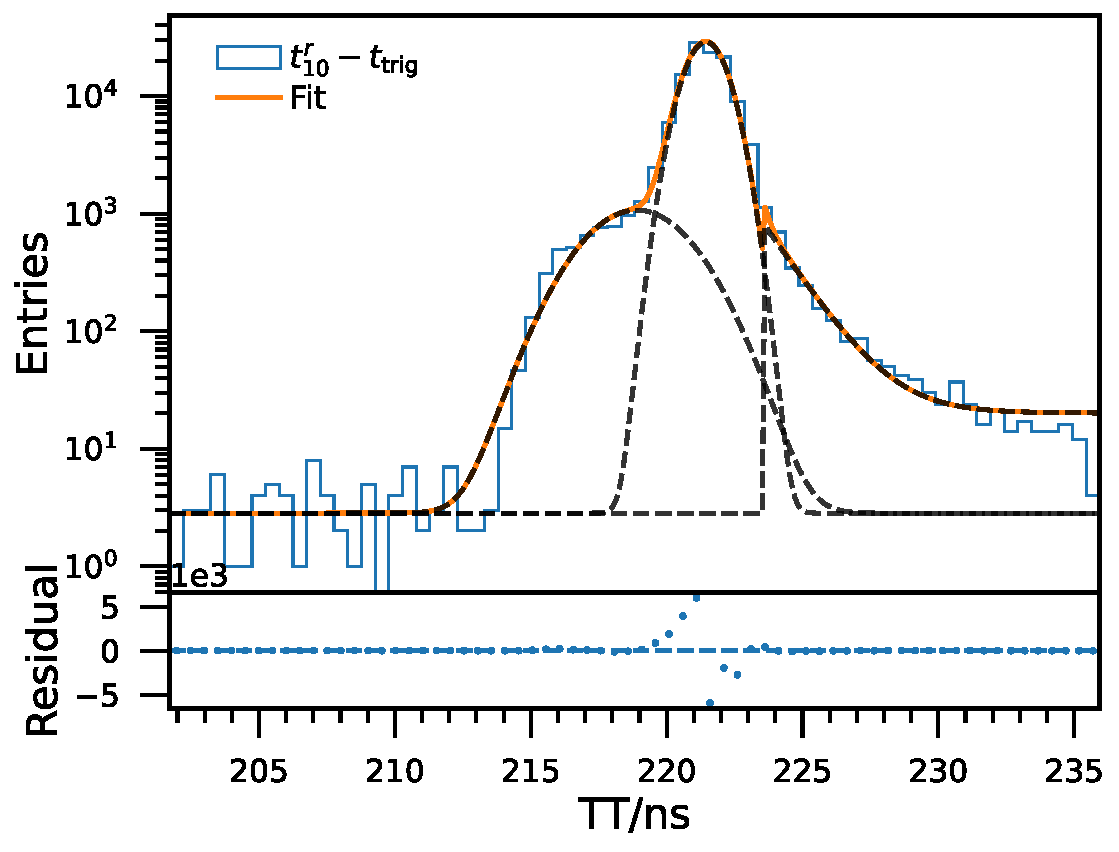
\includegraphics[width=\textwidth]{figures/method/triggerTTSLog.pdf}
        \caption{}%PM
        \label{fig:triggerTTSLog}
    \end{subfigure}
    \begin{subfigure}[t]{\SF\textwidth}
        \includegraphics[width=\textwidth]{figures/method/triggerTTS2d.pdf}
        \caption{}%PM
        \label{fig:triggerTTS2d}
    \end{subfigure}
    \caption{(a) The bottom pad is the distribution of TT with the y-axis in the logarithmic scale. The black dashed lines from left to right are early, main and delayed components with a dark noise pedestal. The top pad is the residual between data and fit in linear scale. (b) The 2D distribution of TT and charge with the colorbar in logarithmic scale.}
\end{figure}

\subsection{Dark count rate}
\label{sec:dcr}
The dark noise mimicking PEs mainly comes from the spontaneous thermionic electrons emitted from the photocathode~\cite{KM3NetTesting}. The dark count rate (DCR) is ${N^{\mathrm{noise}}}/({N^{\mathrm{hit}}T_{\mathrm{DCR}}})$, in which $N^{\mathrm{noise}}$ is the noise count in the interval of $[\SI{-300}{ns},\SI{-150}{ns}]$ relative to the main pulse with $T_{\mathrm{DCR}}=\SI{150}{ns}$ and $N^{\mathrm{hit}}$ is the number of waveforms with main pulses. The DCR of 9 MCP-PMTs is $5.3\pm\SI{1.7}{kHz}$ at room temperature.

\subsection{Pre-pulse and after-pulse}
\label{sec:afterpulse}
Generated from photons hitting the MCP or the first dynode directly rather than the photocathode, \emph{pre-pulses} appear about tens of nanoseconds earlier with smaller amplitudes~\cite{JUNOMassTesting}.

Ions such as \ce{H^+}, \ce{He^+} and \ce{O^+} produced from gaseous impurities in the vacuum bulb by the PEs drift back to the photocathode, generate new electrons and further \emph{after-pulses}~\cite{JUNOMassTesting,Coates_1973}. The delay times of after-pulses are proportional to the square root of the mass-to-charge ratios of the ions~\cite{XENON1TTesting,Coates_1973,afterpulseTime}. %Considering electric field and $\frac{M}{Z}$ of ions, the travel time is in the scale of \si{us}.
\begin{figure}
    \centering
    \includegraphics[width=\LF\textwidth]{figures/method/triggerAfterpulseSchema.pdf}
    \caption{An example waveform for searching pre-pulses and after-pulses. Green and red vertical dashed lines are the trigger time and 10\% of the rising edge of the main pulse $t_r^{10}$, respectively. The gray and orange regions are the intervals for searching after-pulses and pre-pulses.}
    \label{fig:afterpulseSchema}
\end{figure}

The pre-pulses and after-pulses are searched from \SI{10}{ns} before and \SI{200}{ns} after the main pulse. The 10\% rise time $t_r^{10}$ and charge $Q$ of the after-pulse and pre-pulse are calculated in the $[-\SI{10}{ns},\SI{75}{ns}]$ window relative to the peak position, as shown by the violet area in Fig.~\ref{fig:afterpulseSchema}.

The ratios of pre-pulses $R_{\mathrm{pre}}$ and after-pulses $R_{\mathrm{after}}$ are calculated in the time interval [\SI{-100}{ns},\SI{-10}{ns}] ($T_{\mathrm{pre}}=90$\,ns) and [\SI{200}{ns},\SI{9800}{ns}] ($T_{\mathrm{after}}=9600$\,ns) relative to the main pulses respectively as the following equations

\begin{align}
    R_{\mathrm{pre}} = \frac{N^{\mathrm{pre}}}{N^\mathrm{hit}} - \mathrm{DCR}\cdot T_{\mathrm{pre}}\\
    R_{\mathrm{after}} = \frac{N^{\mathrm{after}}}{N^\mathrm{hit}} - \mathrm{DCR}\cdot T_{\mathrm{after}}
\end{align}
in which $N^{\mathrm{pre}}$ and $N^{\mathrm{after}}$ are the number of pre-pulses and after-pulses.  The small $R_{\mathrm{pre}}$ ($3\times10^{-5}\pm1.2\times10^{-4}$) is dominated by DCR at our low-occupancy setup, and $R_{\mathrm{after}}$ of 9 MCP-PMTs is $0.009\pm0.006$.

\begin{figure}[!htbp]
    \centering
    \begin{subfigure}[t]{\LF\textwidth}
        \includegraphics[width=\textwidth]{figures/method/triggerAfterpulse1d.pdf}
        \caption{}%PM
        \label{fig:afterpulse1d}
    \end{subfigure}
    \begin{subfigure}[t]{\LF\textwidth}
        \includegraphics[width=\textwidth]{figures/method/triggerAfterpulse2d.pdf}
        \caption{}
        \label{fig:afterpulse2d}
    \end{subfigure}
    \caption{(a) An example of time distributions of pre-pulses (orange) and after-pulses (blue) for an MCP-PMT, the green line being the Gaussian fits. The blank area around the \SI{0}{ns} is the main pulses not shown in this figure. (b) Charge versus time distribution of pre-pulses and after-pulses. The bright horizontal band at about 100\,$\mathrm{ADC}\cdot \mathrm{ns}$ mainly contains dark noise. The black line is the mean charge of pre/after-pulses in each time bin.}
\end{figure}
% waveform analysis

The distribution of the delay time from $t_r^{10}$ of the main to after-pulse in Fig.~\ref{fig:afterpulse1d} indicates five typical peaks or structures at around \SI{300}{ns}, \SI{400}{ns}, \SI{600}{ns}, \SI{1200}{ns} and \SI{1700}{ns}, time ratio being about $1:\sqrt{2}:\sqrt{4}:\sqrt{16}:\sqrt{32}$. These groups may originate from \ce{H^+}, \ce{H_2^+}, \ce{He^{+}}, \ce{CH_4^+}, and \ce{N_2^+} or \ce{O_2^+}. XENON1T~\cite{XENON1TTesting} and XMASS~\cite{Abe_2020} gave the same assumptions for the first peak. Similar works by JUNO~\cite{Zhao:2022gks} and KM3NeT~\cite{KM3NetTesting} claimed the first peak to be \ce{H_2^{+}}.

We use five Gaussians $\sum_{i=1}^{5}{A_if_i^{\mathrm{AP}}(t;t_i,\sigma_i^2)}$ to model the five groups after subtracting DCR, in which $A_i$, $t_i$, and $\sigma_i$ are the amplitudes, times, width of each after-pulse group (Table.~\ref{tab:afterpulse}). The amplitudes of the groups vary greatly for different MCP-PMTs in Fig.~\ref{fig:afterpulsePeak}. Besides, we suggest roughly modeling the time and charge distribution of unexplained slow undulating structures contributing about half of the after-pulses on average in the time interval $[\SI{2000}{ns},\SI{7000}{ns}]$, as shown in Fig.~\ref{fig:afterpulse1d}, with the uniform time and the single PE charge distribution.

\begin{table}
    \centering
    \caption{Parameters of after-pulse of MCP-PMTs}
    \label{tab:afterpulse}
    \begin{threeparttable}
        \begin{tabular}{c|c|c|c|c|c}
            \hline
            &1st group&2nd group&3rd group&4th group&5th group\\
            \hline
            $t_i$/ns&310$\pm$8&435$\pm$27&593$\pm$24&1201$\pm$41&1725$\pm$25\\
            $A_i/N^{\mathrm{hit}}$(/1E3)&1.2$\pm$0.7&0.3$\pm$0.2&0.3$\pm$0.3&0.8$\pm$0.6&1.5$\pm$0.6\\
            $\sigma_i$/ns&15$\pm$6&40$\pm$16 &32$\pm$12&50$\pm$26&68$\pm$23\\
            $Q_i/Q_0$&32$\pm$3&32$\pm$3\tnote{1}&20$\pm$3&17$\pm$3&14$\pm$1\\
            $\sigma_{Q_i}/Q_0$&12$\pm$1&12$\pm$1\tnote{1}&21$\pm$7&9$\pm$1&8$\pm$1\\
            \hline
        \end{tabular}
        \begin{tablenotes}
            \footnotesize
            \item[1] The charge parameters of the 2nd group inherit from the 1st group.
        \end{tablenotes}
    \end{threeparttable}
\end{table}

\begin{figure}[!htbp]
    \centering
    \begin{subfigure}[t]{\SF\textwidth}
        \includegraphics[width=\textwidth]{figures/result/afterpulse.pdf}
        \caption{}%PM
        \label{fig:afterpulsePeak}
    \end{subfigure}
    \begin{subfigure}[t]{\SF\textwidth}
        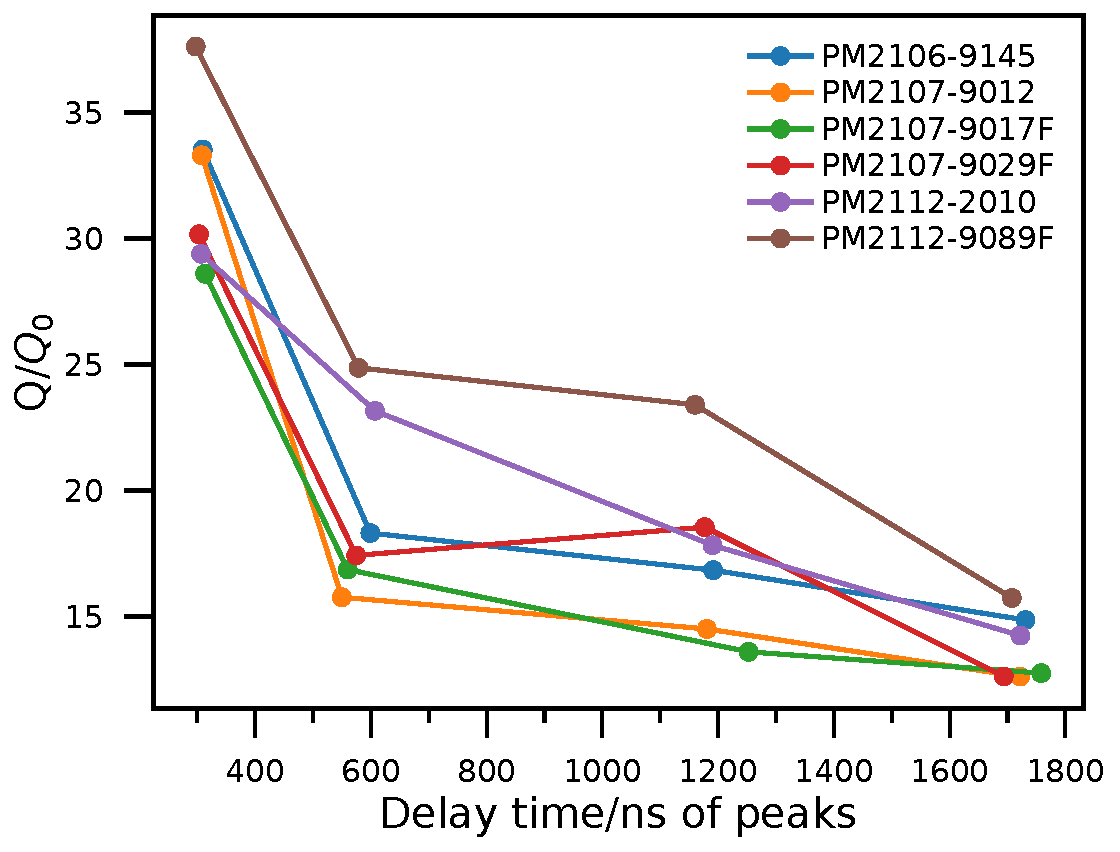
\includegraphics[width=\textwidth]{figures/result/afterpulseQ.pdf}
        \caption{}%PM
        \label{fig:afterpulseQ}
    \end{subfigure}
    \caption{(a) Time and relative amplitudes of after-pulse groups of 9 MCP-PMTs. (a) Time and mean charge of after-pulse groups of 6 MCP-PMTs.}
\end{figure}

%The mean charge in each time bin shown as the black line. 
The after-pulse groups contain large charge signals, as shown in Fig.~\ref{fig:afterpulse2d}. The charge distributions in $[t_i-3\sigma_i,t_i+3\sigma_i]$ of each after-pulse group except for the 2nd one are scaled to the same dark noise count in Fig.~\ref{fig:afterpulsecharge}. We suggest using the same charge parameters with the 1st group for the 2nd group due to overlap with the 1st. The low charge area is consistent with dark noise, and the large charge events contributed from after-pulses are fitted with a Gaussian $f^{AP_Q}_i(Q;Q_i,\sigma_{Q_i}^2)$, in which $Q_i$ and $\sigma_{Q_i}$ are the charge and spread of each after-pulse group (Table.~\ref{tab:afterpulse}). The mean charge of each group without the 2nd one of six high statistics PMTs in Fig.~\ref{fig:afterpulseQ} shows a negative correlation between charge and delay time. The charge distribution of 3rd low statistics group cannot be fitted well and therefore $\sigma_{Q_3}$s are large. 

\begin{figure}[!htbp]
    \centering
    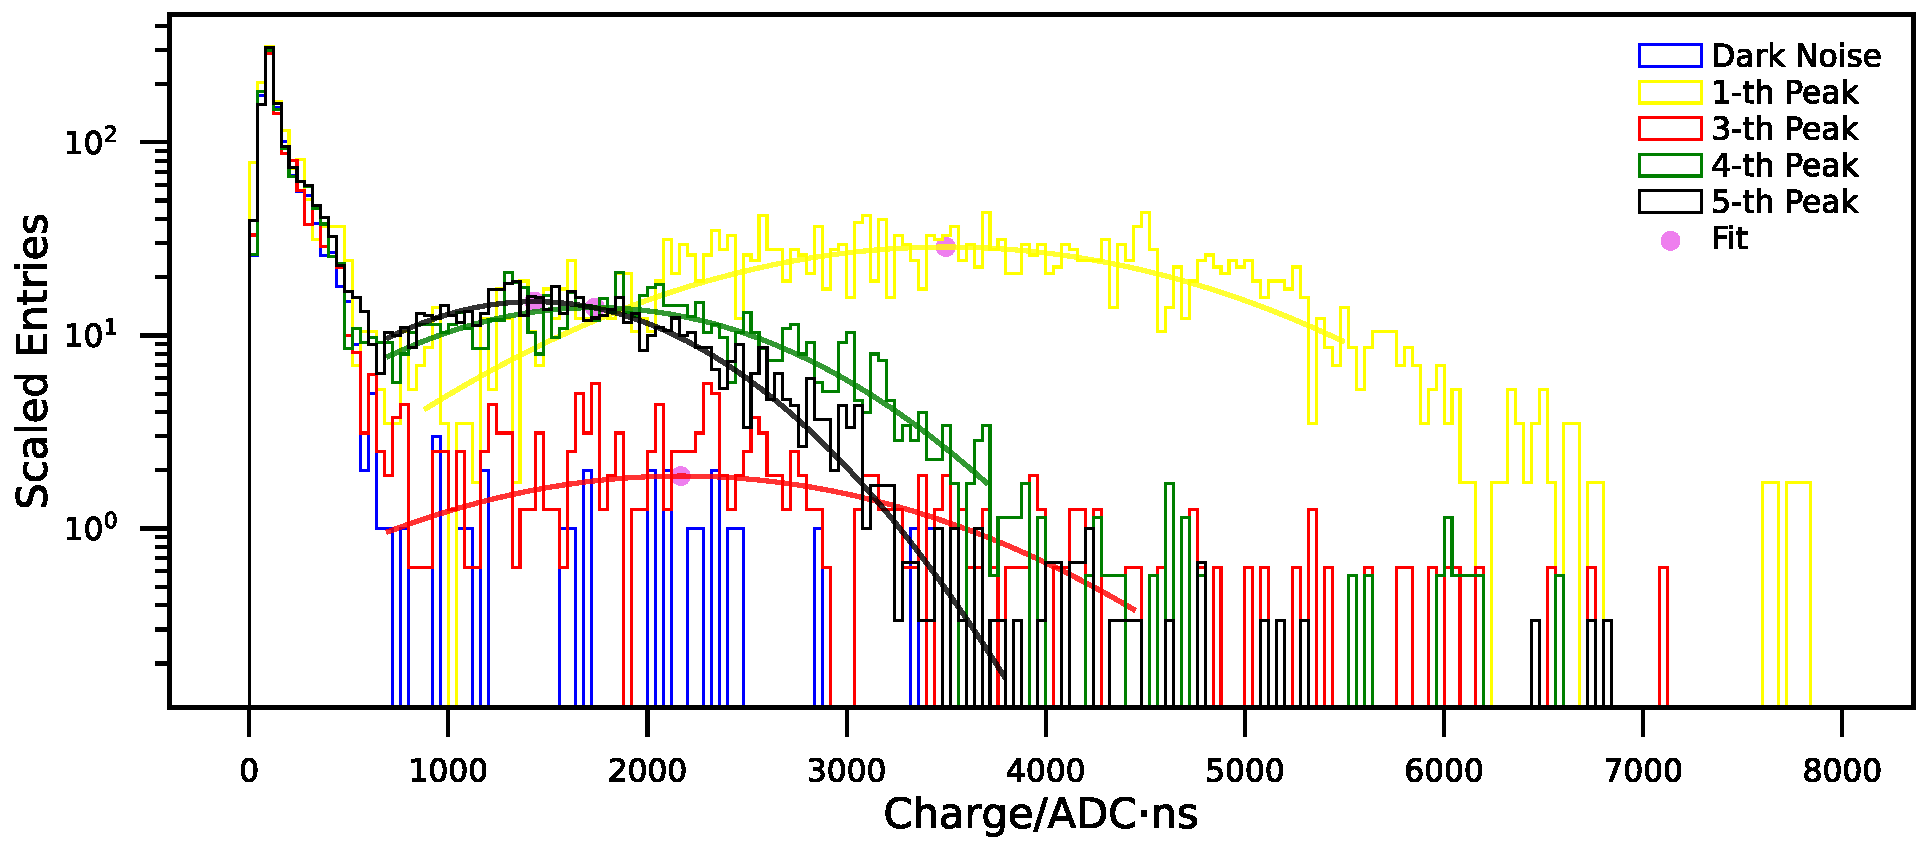
\includegraphics[width=\textwidth]{figures/method/triggerafterpulseCharge.pdf}
    \caption{The charge distribution of after-pulse groups of an example MCP-PMT. The blue histogram is the distribution of dark noise. The violet points are the peaks of fit curves.}
    \label{fig:afterpulsecharge}
\end{figure}

\subsection{Relative photon detection efficiency}
\label{sec:PDE}
 %For example, JUNO fixed one reference PMT to calibrate the light intensity and other reference PMTs are circulated through all channels to calibrate the light allocation ratio~\cite{Wonsak_2021}.
A regression method is developed to combine the light-source calibration and PDE measurements simultaneously. Note $I_n$ to be the light intensity of the $n$th run, $\alpha_j$ to be the light allocation ratio of the $j$th splitter channel (out of four and assumed to be stable across runs), $\eta_k$ to be the PDE of the $k$th PMT (out of one reference dynode and nine MCP PMTs). The PE counts in each waveform obey Poisson distribution $\pi(I_n\alpha_j\eta_k)$.

For convenience, the index of the reference PMT is set to 0. Note $\alpha_j^0\equiv\alpha_j/{\alpha_0}$, $\eta_k^0\equiv\eta_k/{\eta_0}$, $I_n^0\equiv I_n\alpha_0\eta_0$.  The hit rate $R_{njk}$ of the $k$th PMT at the $j$th channel in the $n$th run is

\begin{equation}
    \label{equ:linkfunction}
    R_{njk}=1-\exp\left(-I_n\alpha_j\eta_k\right)=1-\exp\left(-e^{\log{I_n^0}+\log{\alpha_j^0}+\log{\eta_k^0}}\right).
\end{equation}

The number of hit waveforms $N^{\mathrm{hit}}_{njk}$ of the $k$th PMT in the $n$th run with the $j$th channel obeys Binomial distribution $B(N^{\mathrm{hit}}_{njk};R_{njk},N^t_{njk})$, in which $N^t_{njk}$ is the total number of waveforms by the laser trigger. The likelihood is therefore

\begin{equation}
    \label{equ:likelihood}
    \mathcal{L}=\prod_{njk}{R_{njk}^{N^\mathrm{hit}_{njk}}(1-R_{njk})^{N^t_{njk}-N^{\mathrm{hit}}_{njk}}}.
\end{equation}

Eqs.~\eqref{equ:linkfunction} and \eqref{equ:likelihood} defines a \emph{Binomial regression} with \emph{complementary log-log} link function~\cite{glm}, with $\log{\eta_k^0}$, $\log{\alpha_j^0}$ and $\log{I_n^0}$ as parameters. The relative PDEs $\eta_k^0$ of MCP-PMTs are calculated from the regression results to be about $1.71$, significantly higher than the reference PMT.  We could attribute the PDE to the improvements on both quantum and collection efficiencies of the MCP-PMTs. 

\section{Testing and characterization}
\label{Result}

\subsection{Noise stage}
The window size is \SI{600}{ns}. For 20kHz dark noise rate, the expected dark noise pulse number is 0.012, which means the probability of 2 or more pulse is about 0.012 of probability of 1 pulse. The maximum peak in each waveform are extracted as the noise pulse candidates.
\subsubsection{Baseline}
Due to the offset mentioned in sec~\ref{sec:setup}, the ADC value of baseline is about 950. To get baseline, the pulse area should be removed. A procedure to determine the baseline is developed, which comprised three steps and shown in Fig~\ref{fig:baseline1}
\begin{figure}[!htbp]
    \centering
    \begin{subfigure}[b]{\textwidth}
        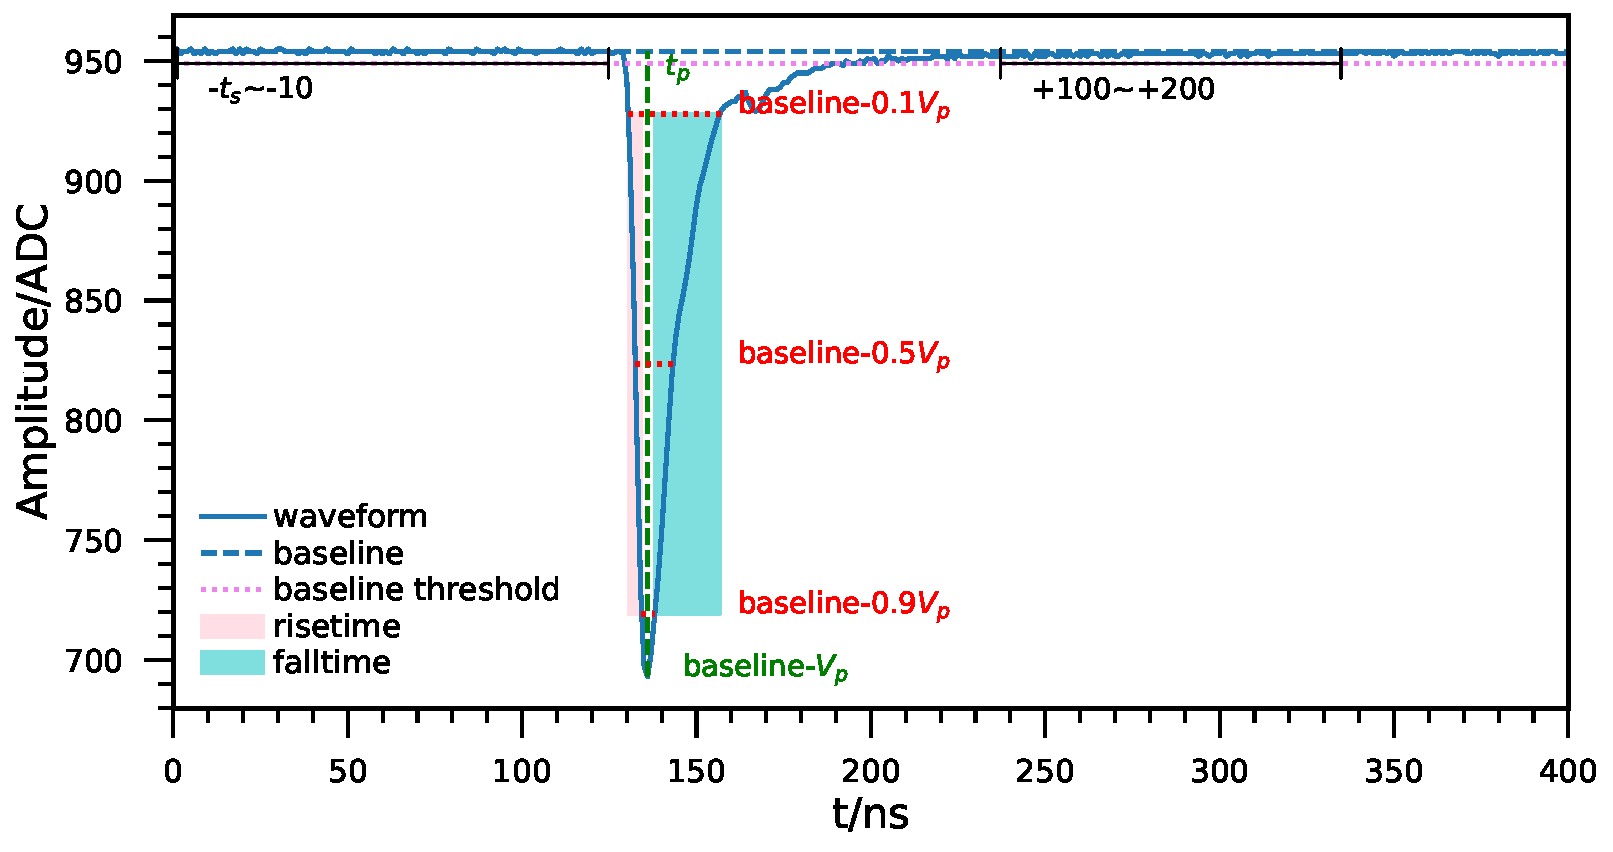
\includegraphics[width=\textwidth,page=1]{figures/result/noisebaseline697_219908_2.pdf}
        \caption{An example of waveform in noise stage}
        \label{fig:baseline1}
    \end{subfigure}
    \begin{subfigure}[b]{\textwidth}
        \includegraphics[width=\textwidth,page=3]{figures/result/noisebaseline697_219908_2.pdf}
        \caption{An example of waveform without baseline in noise stage}
        \label{fig:baseline2}
    \end{subfigure}
\end{figure}

1. An interval in the time window $[-t_s,-10]$ ($t_s\in[-200,-110]$) ns relative to pulse peak $t_p$ is selected. If $t_s<110$ when the peak is close to the start of waveform, another interval $[100,200]$ ns relative to $t_p$ is appended to expand the total interval. Average $\mu_b^0$ and standard deviation $\sigma_b^0$ of amplitudes are calculated.

2. An amplitude filter $[\mu_b^0-\max(\min(5\sigma_b^0,3),1)]$ is used to remove most of signal and reserve the baseline when $\sigma_b^0$ is small.

3. The rest amplitudes are fitted with a gaussian function G$(\mu_b^f,\sigma_b^f)$ using unbinned likelihood. $\mu_b^f$ and $\sigma_b^f$ are accurate at most time. When there exsit a large wave in the time interval selected in step1, a bias will be introduced for $\sigma_b^f$ which can be seen in Fig~\ref{fig:baselineBias2}.

4. Another amplitude filter $[\mu_b^f-\min(5\sigma_b^f,3)]$ is used to reselect the signal area and those areas are padding \SI{10}{ns} to remove rising edge and falling edge. The rest wave are used to estimate baseline $\mu_b$ and standard deviation of baseline $\sigma_b$.
\begin{figure}[!htbp]
    \centering
    \begin{subfigure}[b]{0.7\textwidth}
        % \includegraphics[width=0.8\textwidth]{figure/facility/facility.pdf}
        \caption{Peak distribution of an example PMT}%PM
        \label{fig:baselineBias1}
    \end{subfigure}
    \begin{subfigure}[b]{0.3\textwidth}
        % \includegraphics[width=0.8\textwidth]{figure/facility/facility.pdf}
        \caption{An example of waveform in noise stage}
        \label{fig:baselineBias2}
    \end{subfigure}
\end{figure}

\subsubsection{Peak and charge spectrum}
\label{sec:noisepeak}
The charge of pulses is calculated using integration in a time window $[-15, 75]$ ns relative to the peak location $t_p$ of the signal (Fig~\ref{fig:baseline2}) considering the rise time and fall time distribution. There exist a long tail in charge distribution. A gaussian function is used to fit the binned data via modified least-square method to get the peak of single PE. A parabolic function is fitted to the vally interval as shown in Fig~\ref{fig:charge}.

The peak amplitude distribution is shown in Fig~\ref{fig:peak}
\begin{figure}[!htbp]
    \centering
    \begin{subfigure}[t]{0.45\textwidth}
        \includegraphics[width=\textwidth,page=3]{figures/result/peakcharge697.pdf}
        \caption{Charge distribution of an example PMT}%PM
        \label{fig:charge}
    \end{subfigure}
    \begin{subfigure}[t]{0.45\textwidth}
        \includegraphics[width=\textwidth,page=5]{figures/result/peakcharge697.pdf}
        \caption{ distribution of an example PMT}%PM
        \label{fig:peak}
    \end{subfigure}
    \caption{Peak and charge distribution of an example PMT}
\end{figure}
\subsubsection{Dark count rate}
A float threshold $V_{t}$ as shown in Fig~\ref{fig:peak} was selected as the vally of histogram of peak distributuion to discriminate the dark noise and fluctuation of baseline. The DCR equals to $\frac{N_{\mathrm{noise}}}{N_{t}}$, in which $N_{\mathrm{noise}}$ is the noise number and $N_{t}$ is the total number of waveforms.

\subsection{Laser stage}
The window size is \SI{10400}{ns} and the trigger time is at ~\SI{200}{ns} as shown in Fig~\ref{fig:triggerwaveform}. The trigger pulse are mainly centering in the time interval between [250, 350]ns dependent on the length of cable. The maximum peak are found in the window of [0, 600]ns and extract the peak position. A gaussian function G$(\mu_t^0,\sigma_t^0)$ is fit to the distribution of peak location shown in Fig~\ref{peaklocation}. A time cut $[\mu_t^0-3\sigma_t^0, \mu_t^0+3\sigma_t^0]$ is used for the waveforms dataset of each PMTs. All the characterizations are recalculated with the new time cut.

In order to yield SPE events as signal the laser intensity was adjusted to a level where only
about one out of 20 trigger signals led to a PMT signal.

\begin{figure}
    \centering
    \begin{subfigure}[b]{0.35\textwidth}
        % \includegraphics[width=0.8\textwidth]{figure/facility/facility.pdf}
        \caption{An example of waveform in laser stage}
        \label{fig:triggerwaveform}
    \end{subfigure}
    \begin{subfigure}[b]{0.35\textwidth}
        % \includegraphics[width=0.8\textwidth]{figure/facility/facility.pdf}
        \caption{peak location distribution of an example PMT}%PM
        \label{fig:peaklocation}
    \end{subfigure}
    \caption{Peak and charge distribution of an example PMT}
\end{figure}
\subsubsection{Stability of intensity of laser}
\subsubsection{Peak and charge spectrum}
\label{sec:triggerpeak}
The peak and charge calculation method are same as above in sec~\ref{sec:noisepeak}.

The peak amplitude distribution is shown in Fig~\ref{fig:triggerpeak}. The charge distribution with amplitude cut is shown in Fig~\ref{fig:triggercharge}.
\begin{figure}[!htbp]
    \centering
    \begin{subfigure}[b]{0.35\textwidth}
        % \includegraphics[width=0.8\textwidth]{figure/facility/facility.pdf}
        \caption{Peak distribution of an example PMT}%PM
        \label{fig:triggerpeak}
    \end{subfigure}
    \begin{subfigure}[b]{0.35\textwidth}
        % \includegraphics[width=0.8\textwidth]{figure/facility/facility.pdf}
        \caption{Charge distribution of an example PMT}%PM
        \label{fig:triggercharge}
    \end{subfigure}
    \caption{Peak and charge distribution of an example PMT}
\end{figure}
The results of noise and trigger methods are consist.
\subsubsection{Gain and single PE resolution}
Due to the charge distribution contains a long tail, a guassian function G$(G_1,\sigma_{G1})$ is fit to the main peak with cut between . The gain $G$ is calculated as following equation
\begin{equation}
    G=\frac{Q_1}{Q_{\mathrm{ped}}}
\end{equation}
in which $Q_{\mathrm{ped}}$ is set as 0.
\subsubsection{Peak-to-valley(P/V) ratio}
The local minimum $N_v$ of charge spectrum between pedestal and SPE peak is fitted by a parabolic function. The $N_p$ is the peak fitted with gaussian function described in sec~\ref{sec:triggerpeak}.
The peak-to-valley ratio is equal to  
\begin{equation}
    P/V=\frac{N_p}{N_v}
\end{equation}
The P/V show the ability of discrimination between electronic noise and true signal. The results shows P/V of MCP PMTs are better than reference PMT.
\subsubsection{rise time, fall time and full width at half maximum(FWHM)}
The definitions of rise time, fall time and FWHM are shown in Fig~\ref{fig:waveform}($t_{10}, t_{90}$ are the time of 10\% and 90\% amplitude). Fig~\ref{fig:FWHM} shows the distribution of a PMT.
\begin{figure}
    % \includegraphics[width=0.8\textwidth]{figure/facility/facility.pdf}
    \caption{An example of FWHM in noise stage}
    \label{fig:FWHM}
\end{figure}
\subsubsection{Transit time spread (TTS)}
The transit time spread (TTS) is the spread of photo-electron transit time (TT), which represents resolution of timing. The transit time cannot be measured directly, while the trigger time of laser and time of pulse can be measured. A relative transit time ($\mathrm{TT}_r$) is definited as the time between trigger time and $t_{10}^r$. A gaussian fuction G$(\mu_t,\mathrm{TTS}^2)$ is fitted to the distribution of $\mathrm{TT}_r$.
\subsubsection{Single electron response (SER)}
All the waveform from the the charge cut [] are align with $t_{10}^r$ and average to get the SER.
\subsubsection{Pre-pulse and after-pulse}
Pre-pulses generate due to photons hit on the MCP or the first dynode directly rather than the photocathode\cite{JUNOMassTesting}. The amplitude of pre-pulses are smaller than normal signal and appear before the main pulse. This ratio is related to the intensity of light source.
% waveform analysis
Afterpulse are generated due to the ionization of gaseous impurities between the cathode and first dynode when photo-electrons go through\cite{Coates_1973}. These ions hit back on the photocathode and generate electrons. $H^+,He^+,O^+$ are the major ions contributing to afterpulse\cite{Coates_1973}. Due to these ions are heavy than electron, the travel time is in the scale of \si{us}\footnote{The velocity of ions is about \SI{1000}{km/s} and size of PMT is about \SI{0.1}{m}, thus the transit time is about \SI{0.1}{us}}. The after pulse is calculated in a window \SIrange{300}{10000}{ns} after the main pulse.


Afterpulse is categorized into several kinds. Fig~\ref{fig:afterpulse} indicates serveral typical after-pulse peaks in time around \SI{1000}{ns} with ratio about xx\%. Considering the different mass of ions, these peaks originates from xx, xx.
\subsubsection{relative photon detection efficiency}
To measure PDE, the intensity of light and light allocation ratio of each channel need to be calibrated. For example JUNO fixed one reference PMT and other reference PMTs are circulated through all channels \cite{Wonsak_2021}. A new method is designed to reduce the number of reference PMT and combine all test runs to do calibration.  

Note $n,j,k$ ($n=0,...,N-1, j=0,...,J-1, k=0,...,K-1$) is the indicator of test run, channel of splitter and PMT. Intensity of light is $I_n$, light allocation ratio is $\alpha_j$ and photon detection efficiency is $\eta_k$. Assume $\alpha_j$s are stable among different test runs. The trigger rate of nth run, kth PMT in jth channel is
\begin{equation}
    \label{equ:pderate}
    R_{njk}=I_n\alpha_j\eta_k
\end{equation}
For convenience, 0th PMT is the reference PMT. Note $\alpha_j^0=\frac{\alpha_j}{\alpha_0}$, $\eta_k^0=\frac{\eta_k}{\eta_0}$, $I_n^0=I_n\alpha_0\eta_0$, Equ~\eqref{equ:pderate} can be transfer to Equ~\eqref{equ:pdelograte}
\begin{equation}
    \label{equ:pdelograte}
    \mathrm{log}(R_{njk})=\mathrm{log}(I_n^0)+\mathrm{log}(\alpha_j^0)+\mathrm{log}(\eta_k^0)
\end{equation}
Equ~\eqref{equ:pdelograte} is a equation set with $NK$ equations. $I_n^0,\alpha_j^0,\eta_k^0$ are the unknown $N+K+J-2$ parameters, which can stacked into an array $X = C(\mathrm{log}(I_n^0), \mathrm{log}(\alpha_j^0),\mathrm{log}(\eta_k^0))$ ($n=0,...,N-1, j=1,...,J-1, k=1,...,K-1$). 
\begin{equation}
    \mathrm{log}(R_{njk})=DX
\end{equation}
in which $D=[D_I,D_\alpha, D_\eta]$ is a sparse matrix, $D_I[{njk},n]=1,D_\alpha[{njk},j-1]=1, D_\eta[{njk},k-1]=1$. 
In Appendix~\ref{sec:solution} there exist solution only when the  equation set
\section{Summary}
\label{Summary}
The characteristics of 9 MCP-PMTs are measured in this work, which can be used for simulation and further research. A new calibration method for PDE is developed and the expected relative PDE of the new type 8-inch MCP-PMT is significantly high and is about 1.7 times higher than the reference PMT. Although the long tail in the charge distribution worsen \emph{sample resolution}, the ability for boosting energy resolution is promising.
\section{Acknowledgments}
This work is supported in part by the National Natural Science Foundation of China (11620101004), the Key Laboratory of Particle \& Radiation Imaging (Tsinghua University). 

\bibliographystyle{elsarticle-num-names}
\bibliography{introduction,facility,method,result}
% \appendix
% \section{Weighted least square(WLS) for PDE}
\label{sec:solution}
\subsection{Single reference PMT}
\label{sec:singlepmt}
When the PMTs rotate in container for K times, $N=K$ and matrix D contains $NK=K^2$ rows:
\begin{equation}
    \bordermatrix{
        k&I&\alpha&\eta\cr
        0&\mathrm{I}_{(N,N)}&A_{0}&E_{0}\cr
        \vdots&\vdots&\vdots&\vdots\cr
        K-1&\mathrm{I}_{(N,N)}&A_{n}&E_{n}
    }
\end{equation}
in which $A_n$ and $E_n$ are in shape $(K,K-1)$. $A_n$ meet the condition $\sum_i{A_n[i,j]}=1$
\begin{equation}
    A_0=\begin{pmatrix}
        0\\
        I_{(K-1,K-1)}
    \end{pmatrix}
\end{equation}
and $A_n$ are the row arrangement of $A_0$ dependent on the test setting.

Due to the arrangement of $A_n$, each $A_n$ represent all test data for one PMT, therefore $E_n$ should match $A_n$ and all elements are 0 for $E_0$ or contans a column of 1.
\begin{equation}
    E_1=\begin{pmatrix}
        1&0&\dots&0\\
        \vdots&0&\ddots&0\\
        1&0&\dots&0
    \end{pmatrix}
\end{equation}
$E_n$ meet the condition $\sum_n{\sum_i{E_n[i,j]}}=J$.

Above is a special case when all tests contain same PMTs. The number of parameter must be smaller than equations, which lead to $(N-2)(K-1)\geq0$. This methods can be extends to more complicates situation, for example different runs may contain different PMTs. However, there are some limits. If no pmts are include in two different runs sets, $X$ can be split into 5 groups $X=[X_\alpha, X^1_I,X^2_I,X^1_\eta,X^2_\eta]$. The matrix D can be diagonalized into 3 matrix. 
\begin{equation}
    \begin{pmatrix}
        D^1_\alpha&D^1_I&D^1_\eta&0&0\\
        D^2_\alpha&0&0&D^2_I&D^2_\eta
    \end{pmatrix}
\end{equation}
Assume reference PMT exists in 1st group, if there exisit a solution or solution for minimum likelihood $[x_\alpha,x^1_I,x^2_I,x^1_\eta,x^2_\eta]$, $[x_\alpha,x^1_I,x^1_\eta,kx^2_I,x^2_\eta/k]$ will also be the solution, which means the $X^2_\eta$ can not be calculated.
\subsection{Two reference PMTs}
Assume one reference PMT fixed in 0th channel, the other reference PMT moved with test PMTs. Note the fixed reference PMT is Kth PMT, ids of other PMTs are same as . Matrix D contains $N(K+1)$ rows:
\begin{equation}
    \bordermatrix{
        k&I&\alpha_f\eta_f&\alpha_m&\eta_m\cr
        K&\mathrm{I}_{(N,N)}&1&0&0\cr
        0&\mathrm{I}_{(N,N)}&0&A_{0}&E_{0}\cr
        \vdots&\vdots&0&\vdots&\vdots\cr
        K-1&\mathrm{I}_{(N,N)}&0&A_{n}&E_{n}
    }=\begin{pmatrix}
        I&A_f&0\\
        B_m&0&A_m
    \end{pmatrix}
\end{equation}
in which $\alpha_f\eta_f$ is channel ratio multiplied by PDE of fixed PMT. Definition of $A_n$ and $E_n$ are same as Appendix~\ref{sec:singlepmt}. $X$ is splitted into 4 group, $X=[X_I,X^f_\eta,X^m_\alpha,X^m_\eta]$.

Assume PMTs are moved for $J$ times, the PDE $Q_j$ of test PMT can be calculated directly using
\begin{equation}
    \frac{Q_k}{Q_0} = \frac{R_{njk}R_{mJK}}{R_{mj0}R_{nJK}}
\end{equation}
variance of $R$ is Eq.~\eqref{equ:variance}, the relative variance of $\frac{Q_k}{Q_0}$ is $\sum_{i=jk,j0,JK,JK}{\frac{1-p_k}{N_tp_k}}$, in which $N_t$ is number of total events for some run. To get the PDE, a estimator is constructed as 
\begin{equation}
    \hat{\frac{Q_k}{Q_0}}=\frac{1}{N}\sum_j{\frac{R_{njk}R_{mJK}}{R_{mj0}R_{nJK}}}
\end{equation}
The relative variance of $\hat{\frac{Q_k}{Q_0}}$ can be estimated as $\frac{1}{J^2}\sum_k{\frac{1-p_k}{N_tp_k}}$. To be convenience, $p_k$s are close and note $\sigma^2=\frac{1-p_k}{N_tp_k}$, relative variance is $\frac{\sigma^2}{K}$

As for WLS method, the expected value and variance of $log(\hat{\frac{Q_k}{Q_0}})$ is estimated using Eq.~\eqref{equ:solution} and relative variance of $\hat{\frac{Q_k}{Q_0}}$ is estimated as $U=B\Sigma B^T=(D^T\Sigma D)^{-1}$.
\begin{equation}
    D^TD=\begin{pmatrix}
        (K+1)I_{(N,N)} &[1,\dots,1]^T&B_m^TA_m\\
        [1,\dots,1]&K&0\\
        A_m^TB_m&0&A_m^TA_m
    \end{pmatrix}
\end{equation}

In addition,
\begin{equation}
    A_m^TA_m=\begin{pmatrix}
        KI&1\\
        1&KI
    \end{pmatrix},
    A_m^TB_m=\begin{pmatrix}
        1\\
        1
    \end{pmatrix}
\end{equation}
Due to $det(D^TD)=$

If omit the non-diagonal elements, the variance of $\hat{\frac{Q_k}{Q_0}}$ is $\frac{\sigma^2}{K}$.
\end{document}
